\documentclass[a4paper]{article}
\usepackage[utf8]{inputenc}
\usepackage[russian,english]{babel}
\usepackage[T2A]{fontenc}
\usepackage[left=10mm, top=20mm, right=18mm, bottom=15mm, footskip=10mm]{geometry}
\usepackage{indentfirst}
\usepackage{amsmath,amssymb}
\usepackage[italicdiff]{physics}
\usepackage{graphicx}
\graphicspath{{images/}}
\DeclareGraphicsExtensions{.pdf,.png,.jpg}
\usepackage{wrapfig}
\usepackage{float}
\usepackage{subcaption}
\usepackage{enumitem}
\usepackage{pdflscape}
\usepackage{caption}
\usepackage{array}
\captionsetup[figure]{name=Рисунок}
\captionsetup[table]{name=Таблица}

\title{\underline{Отчет о выполненой лабораторной работе 5.2.1 - 5.1.3}}
\author{Воронин Денис, Б04-407}

\begin{document}

\maketitle

\begin{center}
\textbf{\Large Опыт Франка Герца, Эффект Рамзауэра}
\end{center}

\textbf{Аннотация}
В данной работе проводится измерение энергии первого уровня атома гелия методом электронного возбуждения в динамическом и статическом режимах.

\textbf{Цель работы}: Методом электронного возбуждения измерить энергию первого уровня атома гелия в динамическом и статическом режимах.

\section{Теоретические сведения}

Разреженный одноатомный газ (в нашем случае -- гелий) заполняет трёхэлектродную лампу. Электроны, испускаемые разогретым катодом, ускоряются в постоянном электрическом поле, созданным между катодом и сетчатым анодом лампы. Передвигаясь от катода к аноду, электроны сталкиваются с атомами гелия. Если энергия электрона, налетающего на атом, недостаточна для того, чтобы перевести его в возбуждённое состояние (или ионизовать), то возможны только упругие соударения, при которых электроны почти не теряют энергии, так как их масса в тысячи раз меньше массы атомов.


По мере увеличения разности потенциалов между анодом и катодом энергия электронов увеличивается и, в конце концов, оказывается достаточной для возбуждения атомов. При таких -- неупругих -- столкновениях кинетическая энергия налетающего электрона передаётся одному из атомных электронов, вызывая его переход на свободный энергетический уровень (возбуждение) или совсем отрывая его от атома (ионизация).

При увеличении потенциала анода ток в лампе вначале растёт, подобно тому как это происходит в вакуумном диоде (рис. 2). Однако, когда энергия электронов становится достаточной для возбуждения атомов, ток коллектора резко уменьшается. Это происходит потому, что при неупругих соударениях с атомами электроны почти полностью теряют свою энергию и не могут преодолеть задерживающего потенциала между анодом и коллектором. При дальнейшем увеличении потенциала анода ток коллектора вновь возрастает: электроны, испытавшие неупругие соударения, при дальнейшем движении к аноду успевают набрать энергию, достаточную для преодоления зап потенциала.


\begin{figure}[tbh]
	\centering
	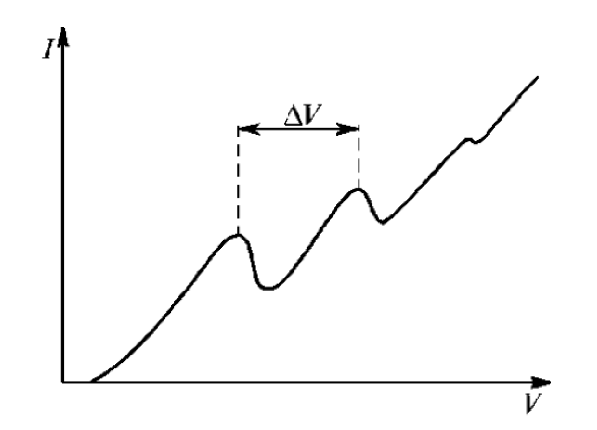
\includegraphics[width=0.4\textheight]{p1.png}
	\caption{Характер зависимости $I (U)$}
	\label{fig:screenshot1}
\end{figure}
\newpage
\subsection{Расчётные формулы}

Кинетическая энергия электрона 1 уровня равна:
\begin{equation}\label{key}
	E = \overline{e} \Delta V \left[эВ\right],
\end{equation}
где $ \Delta V $ -- разность между двумя пиками (см. рис. \ref{fig:screenshot1}).


\[E = \frac{mv^2}{2} = \frac{mv'^2}{2}+U\]

\begin{equation}
n = \frac{\lambda}{\lambda'} = \sqrt{1 - \frac{U}{E}}
\end{equation}

После решения соответствующего уравнения Шрёдингера получается выражение для коэффициента прохождения:

\begin{equation}
D = \frac{16 k_1^2 k_2^2}{16k_1^2 k_2^2 + 4\left(k_1^2-k_2^2\right)^2\sin^2\left(k_2 l\right)}
\end{equation}
где $k_1^2 = \frac{2mE}{\hbar^2}, k_2^2 = \frac{2m(E + U_0)}{\hbar^2}$.

Это периодическое выражение с максимумами при 

\begin{equation}
k_2 l = \pi n = \sqrt{\frac{2m(E + U_0)}{\hbar^2}}l
\end{equation}

Выражения для эффективного размера атома $l$:
\begin{equation}
2l = \frac{h}{\sqrt{2m(E_1 + U_0)}}
\end{equation}

\begin{equation}
2l = \frac{3}{2}\frac{h}{\sqrt{2m(E_2 + U_0)}}
\end{equation}

Где $E_1, E_2$ --- энергии, соответствующие максимуму и минимуму прохождения электронов соответственно. Исключая $U_0$ можно найти 

\begin{equation}
l = \frac{h\sqrt{5}}{\sqrt{32m(E_2 - E_1)}}
\end{equation}

А исключая $l$ можно найти эффективную глубину потенциальной ямы атома:

\begin{equation}
U_0 = \frac{4}{5}E_2 - \frac{9}{5}E_1
\end{equation}

Формула, связывающую зависимость вероятности рассеяния электрона от его энергии:
\begin{equation}
w(V) = -\frac{1}{C} \ln \frac{I_a(V)}{I_0}
\end{equation}


\section{Оборудование и инструментальные погрешности}

Схема экспериментальной установки отображена на рис.4 и 3.

\begin{figure}[H]
\begin{center}
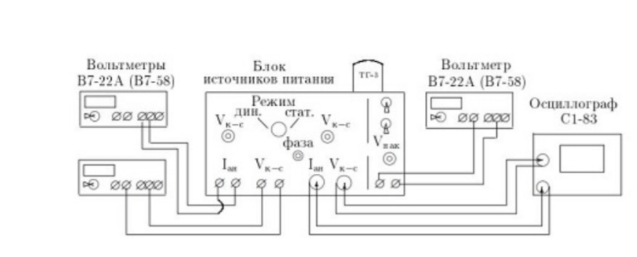
\includegraphics[width = 0.6\textwidth]{p4.png}
\caption{Схема экспериментальной установки}
\end{center}
\end{figure}

\newpage

\begin{figure}[tbh]
	\centering
	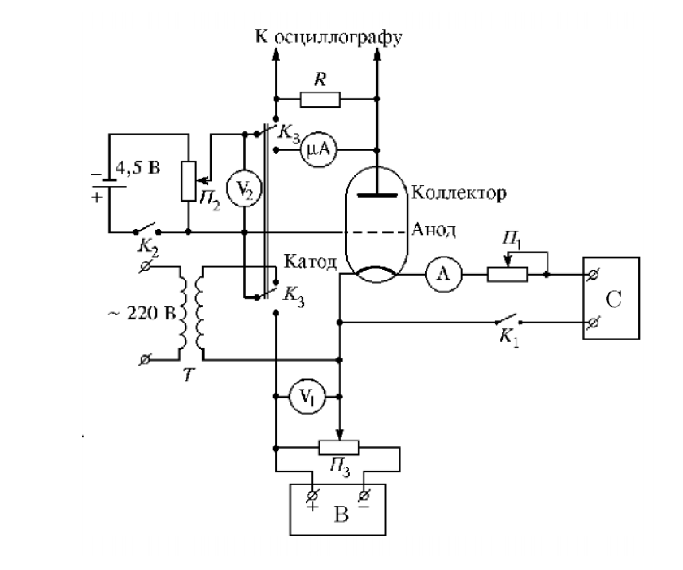
\includegraphics[height=0.4\textheight]{p2.png}
	\caption{Принципиальная схема установки}
	\label{fig:screenshot2}
\end{figure}

\begin{figure}[tbh]
	\centering
	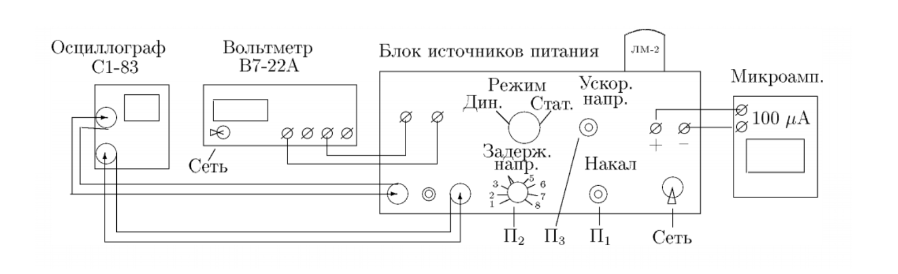
\includegraphics[width=0.6\textheight]{p3.png}
	\caption{Блок-схема экспериментальной установки}
	\label{fig:screenshot3}
\end{figure}




В работе используются:
\begin{itemize}


\item{Осциллограф} $\Delta \pm${0.4}{В} (в данном опыте)
\item{Вольтметр} $\Delta \pm${0.1}{В}
\item{Миллиамперметр}$\Delta \pm${0.5}{мА}
\item{Блок источников питания}
\item {Газонаполненная лампа} (гелий)

\end{itemize}

\newpage

\section{Ход работы}
\subsection{Франк Герц}


\begin{figure}[h]
\begin{center}
\begin{minipage}[h]{0.3\linewidth}
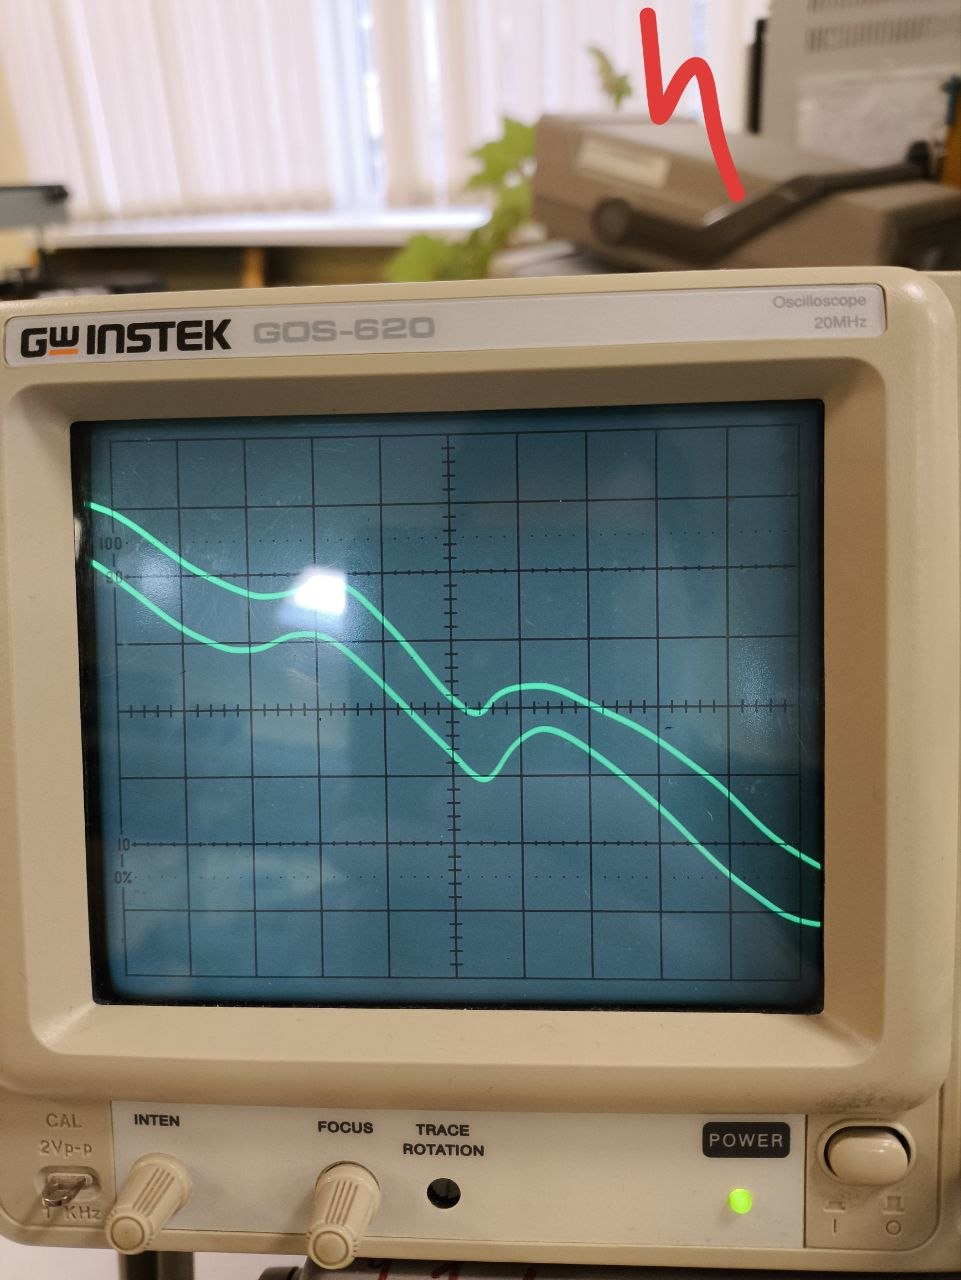
\includegraphics[width=1\linewidth]{4_V.jpg}
\caption{Осциллограмма при задерживающем напряжении 4 В} %% подпись к рисунку
\label{ris:experimoriginal} %% метка рисунка для ссылки на него
\end{minipage}
\hfill 
\begin{minipage}[h]{0.3\linewidth}
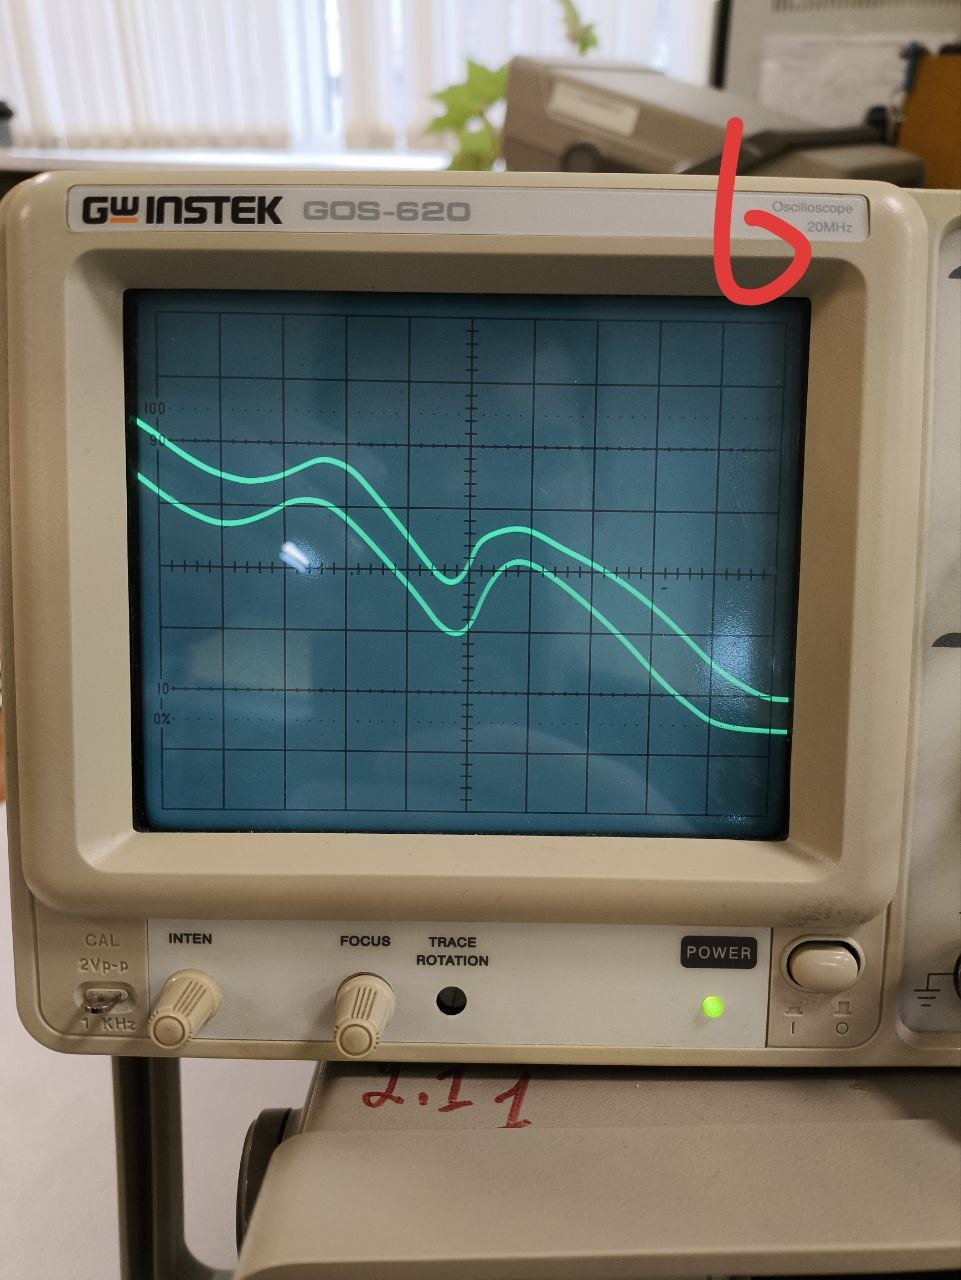
\includegraphics[width=1\linewidth]{6_V.jpg}
\caption{Осциллограмма при задерживающем напряжении 6 В}
\label{ris:experimcoded}
\end{minipage}
\hfill 
\begin{minipage}[h]{0.3\linewidth}
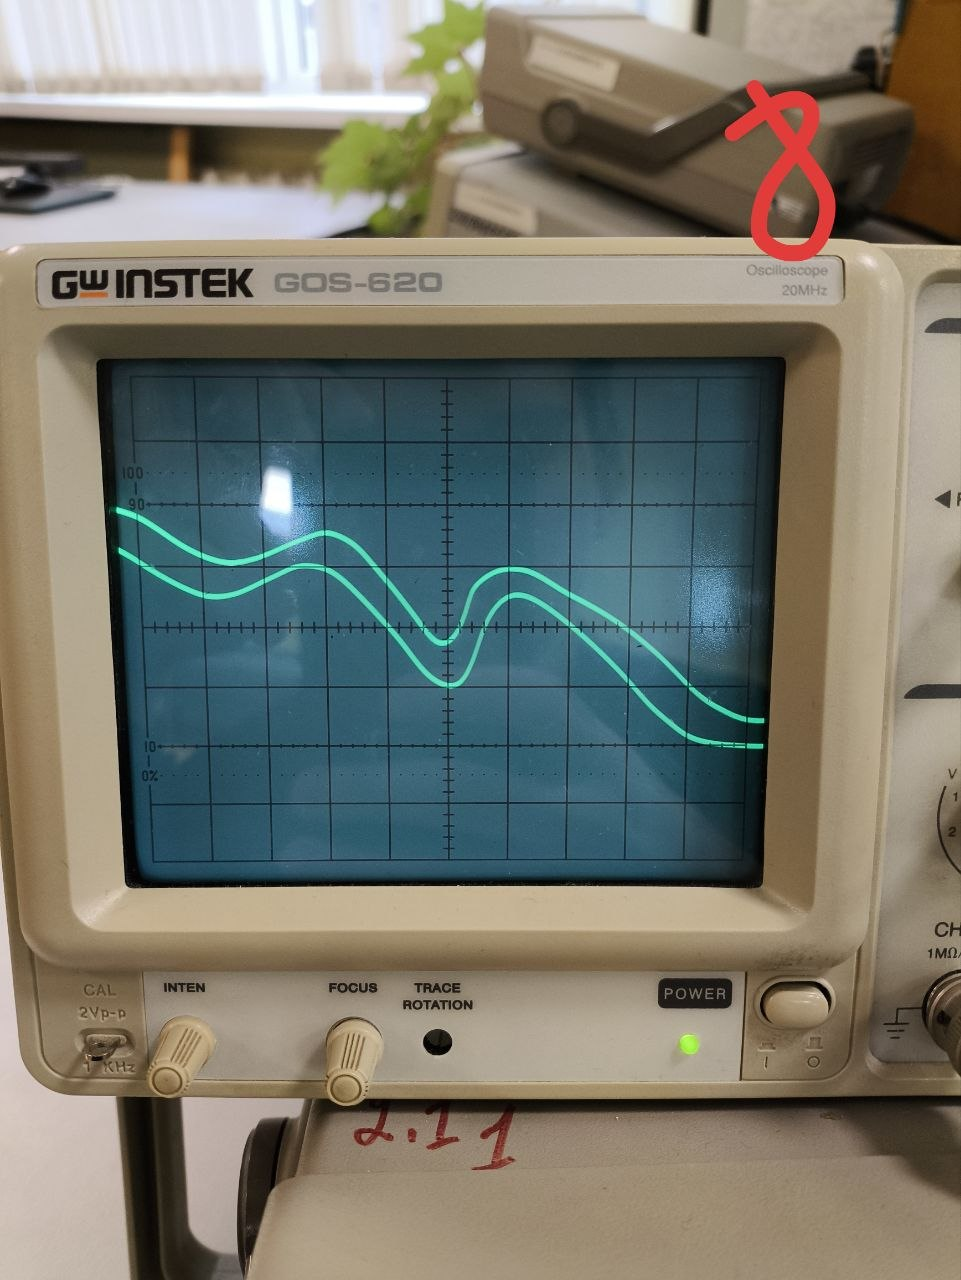
\includegraphics[width=1\linewidth]{8_V.jpg}
\caption{Осциллограмма при задерживающем напряжении 8 В}
\label{ris:experimcoded}
\end{minipage}
\end{center}
\end{figure}

\textbf{Динамический метод}

\begin{itemize}
    \item Цена деления 1 дел = 5 В
    % \item $U_{\text{задерж}}$ = 4 В $\Rightarrow $ 3 дел = 30 В
    % \item $U_{\text{задерж}}$ = 6 В $\Rightarrow $ 2,8 дел = 28 В
    % \item $U_{\text{задерж}}$ = 4 В $\Rightarrow $ 2,6 дел = 26 В
\end{itemize}

\begin{table}[h]
\centering
\begin{tabular}{|l|c|c|c|c|c|c|c|}
\hline
Задерж. напряжение & $V_{max_1}$ & $V_{max_2}$ & $V_{min_1}$ & $V_{min_2}$ & $\Delta V_{max}$ & $\Delta V_{min}$ \\
\hline
4 В & 18 В & 36 В & 23 В & 38 В  & 18 $\pm 1$ В & 15$\pm 1$ В \\
\hline
6 В & 21 В & 38 В & 26 В & 45 В  & 17$\pm 1$ В & 19$\pm 1$ В \\
\hline
8 В & 19 В & 36 В & 25 В & 44 В  & 17$\pm 2$ В & 19$\pm 2$ В \\
\hline
\end{tabular}
\caption{Таблица задержек напряжения}
\label{tab:voltage_delay}
\end{table}

Определим значение энергии первого возбуждённого состояния атома гелия. 
\begin{center}
    $\overline{V_{max}} = 17,3 \pm 2.5$ В \hspace{1cm} $\overline{V_{min}} = 17.6 \pm 2.5$ В
\end{center}
Погрешности определения средних значений 


$\sigma_{V_1}^2 = \sigma_{V_4}^2 + \sigma_{V_6}^2 + \sigma_{V_8}^2$ - погрешность прибора


$\sigma_{V_2} = \sqrt{\frac{1}{6}\sum (V_i - \overline{V})^2}$ 
--- погрешность среднего значения

$\sigma_{V_1} = 2{,}5$ В \hspace{1cm} 
$\sigma_{V_{\max,2}} = 0{,}3$ В \hspace{1cm} 
$\sigma_{V_{\min,2}} = 0{,}4$ В


\[
\Delta_{\text{общ}} = \sqrt{\Delta_{\text{приб}}^2 + \Delta_{\text{сл}}^2} = 2,5 \text{В} 
\]


Среднее значение первого возбуждённого состояния атома гелия по результатам эксперимента:
\begin{center}
    $V_{din} = 17,45 \pm 2,5$ эВ 
\end{center}
При этом табличное значение данной величины составляет
\begin{center}
    $V_{th} = 21.6$ эВ
\end{center}
С учётом погрешности, экспериментальные данные близки к теоретическим.


\textbf{Статический метод}

По полученным данным построим график зависимости I(V)

\newpage

\begin{figure}[tbh]
	\centering
	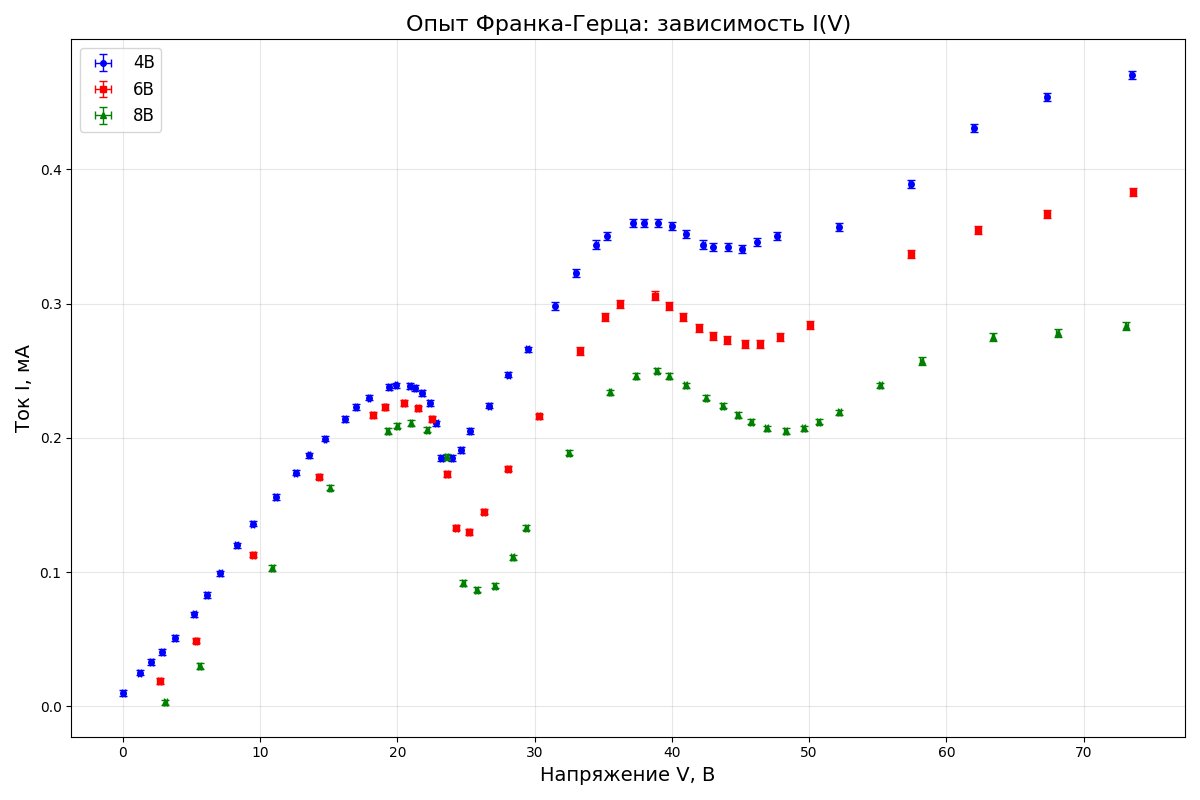
\includegraphics[width=0.6\textheight]{F1.png}
	\caption{Блок-схема экспериментальной установки}
	\label{fig:screenshot3}
\end{figure}

\begin{table}[h]
\centering
\begin{tabular}{|l|c|c|c|c|c|c|c|}
\hline
Задерж. напряжение & $V_{max_1}$ & $V_{max_2}$ & $V_{min_1}$ & $V_{min_2}$ & $\Delta V_{max}$ & $\Delta V_{min}$ \\
\hline
4 В & 20,13 В & 37,83 В & 23,55 В & 44,53 В  & 17,7 $\pm 0,1$ В &21,0 $\pm 0,1$ В \\
\hline
6 В & 20,5 В & 38,3 В & 25,1 В & 45,6 В  & 17,8$\pm 0,1$ В & 20,5$\pm 0,1$ В \\
\hline
8 В & 20,8 В & 38,8 В & 25,9 В & 48,4 В  & 18,0$\pm 0,2$ В & 22,5$\pm 0,2$ В \\
\hline
\end{tabular}
\caption{Таблица задержек напряжения}
\label{tab:voltage_delay}
\end{table}

\begin{center}
    $\overline{V_{max}} = 17,8 \pm 2.5$ В \hspace{1cm} $\overline{V_{min}} = 21,3 \pm 2.5$ В
\end{center}


$\sigma_{V_1} = 0{,}24 $ В \hspace{1cm} 
$\sigma_{V_{\max,2}} = 0{,}2$ В \hspace{1cm} 
$\sigma_{V_{\min,2}} = 0{,}3$ В


\begin{center}
    $V_{stat} = 19,55 \pm 0,44$ эВ 
\end{center}

\textbf{Вывод}


В ходе работы был воспроизведён опыт Франка-Герца, подтверждающий наличие дискретных уровней возбуждения атомов. Вольт-амперная характеристика трёхэлектродной вакуумной лампы была измерена двумя способами - динамическим и статическим. По этим ВАХ были экспериментально определены потенциалы возбуждения атомов гелия 
\begin{itemize}
    \item $V_{din} = 17,45 \pm 2.5$  эВ 
    \item $V_{stat} = 19.55 \pm 0.44$ эВ 
    \item $V_{th} = 21.6 $ эВ
\end{itemize}
Статический метод оказался более точным, чем динамический. \par


\subsection{Рамзауэр}

\textbf{1. Динамический режим}

\newpage

\begin{figure}[tbh]
	\centering
	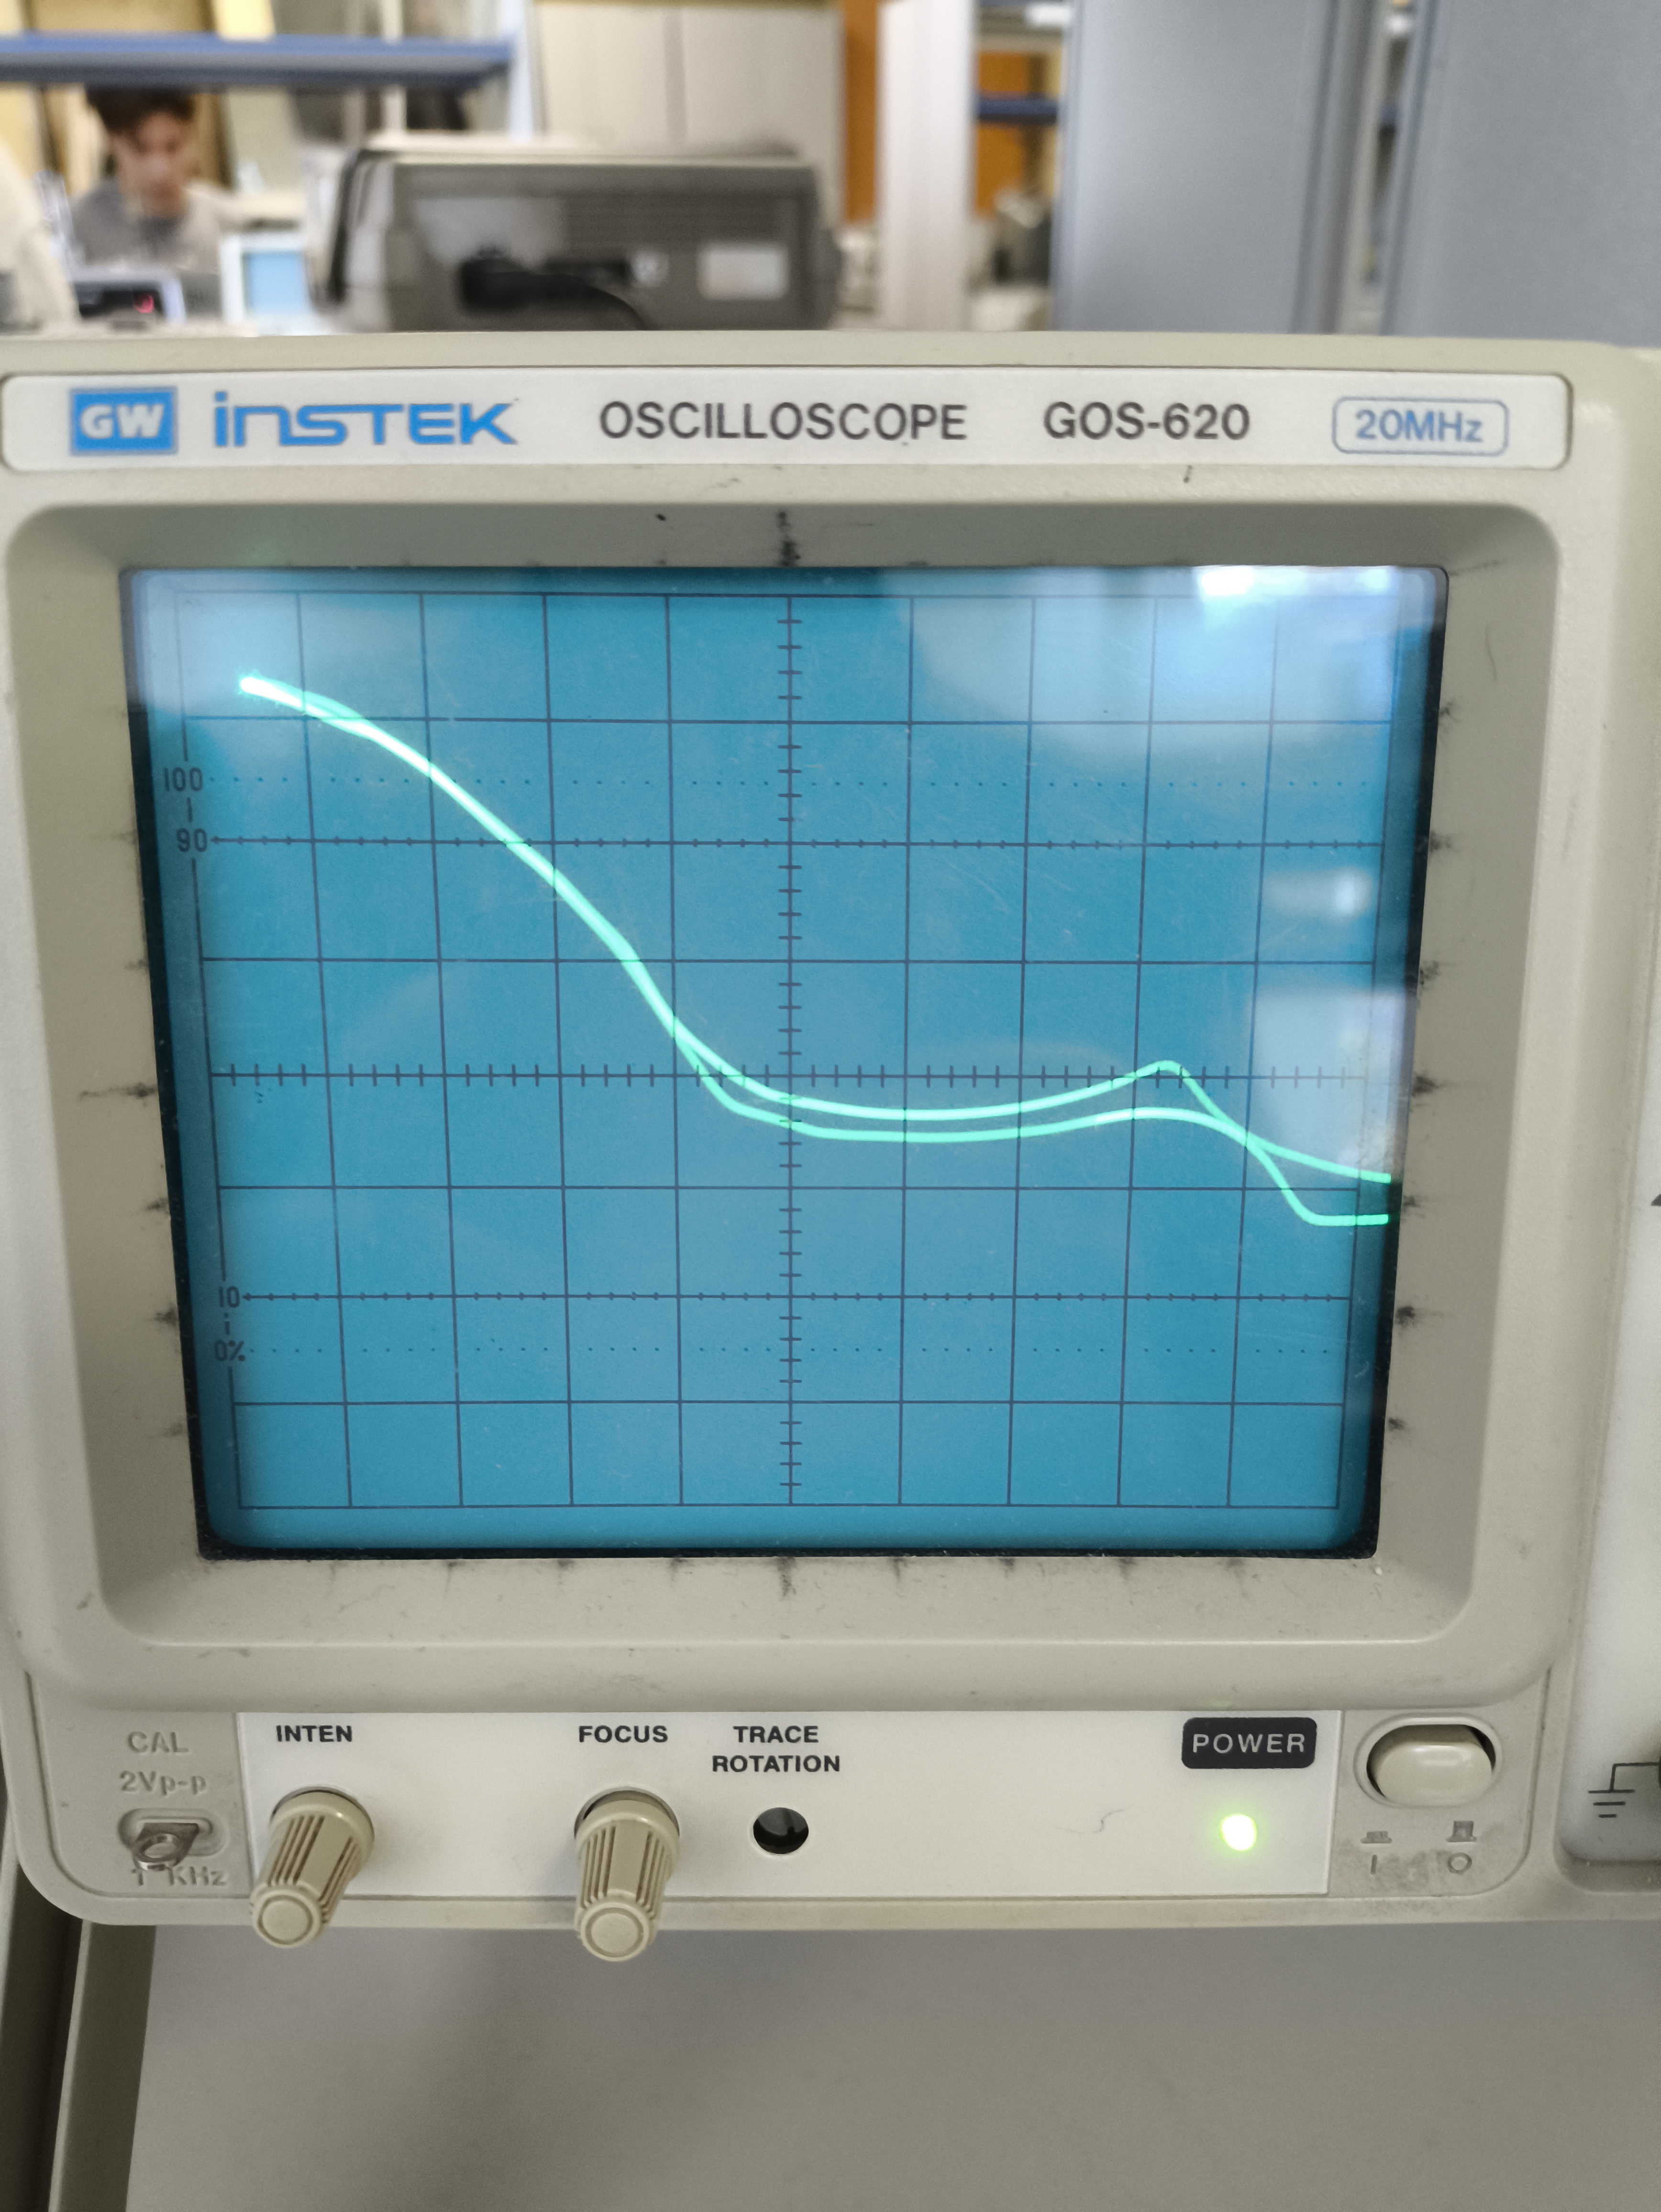
\includegraphics[width=0.2\textheight]{R.jpg}
	\caption{Динамический режим}
	\label{fig:screenshot3}
\end{figure}

\begin{table}[h]
\centering
\begin{tabular}{|c|c|c|}
\hline
 $U_{\text{макс}}$, В & $U_{\text{мин}}$, В & $U_{\text{пробоя}}$, В \\
\hline
 $3{,}8 \pm 0{,}8$ & $8{,}2 \pm 0{,}8$ & $12{,}0 \pm 0{,}8$ \\
\hline
\hline
\end{tabular}
\caption{Характерные значения}
\label{tab:voltage}
\end{table}

Размер оболочки:

\[
l = \frac{h}{2\sqrt{2m_e e(V_{\text{макс.ср}} + U_0)}} = \frac{6{,}626 \cdot 10^{-34}}{2\sqrt{2 \cdot 9{,}109 \cdot 10^{-31} \cdot 1{,}602 \cdot 10^{-19} \cdot 6{,}3}}. = 2,45 \pm 0,03 \text{\AA} \tag{1}
\]
Погрешность
\[
\frac{\Delta l}{l} = \frac{1}{2} \frac{\Delta V_{\text{макс.ср}}}{V_{\text{макс.ср}} + U_0} \approx 0,01
\]
Без учета $U_0$
\[
l' = \frac{h}{2\sqrt{2m_e e V_{\text{макс}}}} \approx 2{,}98~\text{\AA}.
\]

Оба значения (2{,}45~\AA{} и 2{,}98~\AA{}) имеют правильный порядок величины и согласуются с табличными радиусами инертных газов (Ar: 1{,}88~\AA{}, Kr: 2{,}02~\AA{}, Xe: 2{,}16~\AA{}), можно предположить, что газом является Xe.


\textbf{Глубина потенциальной ямы}


\[
U = \frac{\pi^2 \hbar^2}{2 m_e l^2} = 5,16 \hspace{0,1cm} \text{эВ}
\]
% \begin{figure}[tbh]
% 	\centering
% 	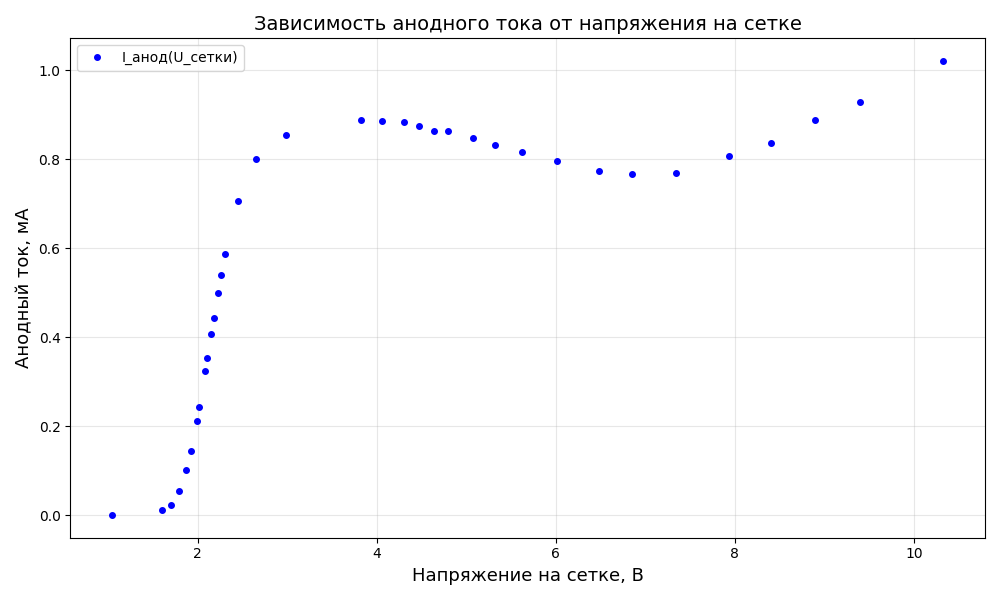
\includegraphics[width=0.6\textheight]{F2.png}
% 	\caption{Статический режим}
% 	\label{fig:screenshot3}
% \end{figure}


\textbf{Потенциал ионизации}

\[
V_{\text{ион}} = V_{\text{проб}} + U_0 = 12 + 2,5 = 14,5 \text{В} \rightarrow 14,5 \text{эВ}
\]

Значит в тиратроне находится Криптон

\textbf{2. Статический режим}

\begin{table}[h]
\centering
\begin{tabular}{|c|c|c|}
\hline
 $U_{\text{макс}}$, В & $U_{\text{мин}}$, В & $U_{\text{пробоя}}$, В \\
\hline
 $3{,}8 \pm 0{,}8$ & $7{,}1 \pm 0{,}8$ & $8{,}5 \pm 0{,}8$ \\
\hline
\hline
\end{tabular}
\caption{Характерные значения}
\label{tab:voltage}
\end{table}


\[
l = \frac{h}{2\sqrt{2m_e e(V_{\text{макс}} + U_0)}} = 2,45 \pm 0,03 \text{\AA} 
\]

\[
l' = \frac{h}{2\sqrt{2m_e e V_{\text{макс}}}} \approx 2{,}98~\text{\AA}.
\]

\[U = 5,16 \text{эВ} \hspace{1cm} V_{\text{ион}} = 11 \text{эВ} \rightarrow \text{Ксенон}\]

\newpage

\begin{figure}[tbh]
	\centering
	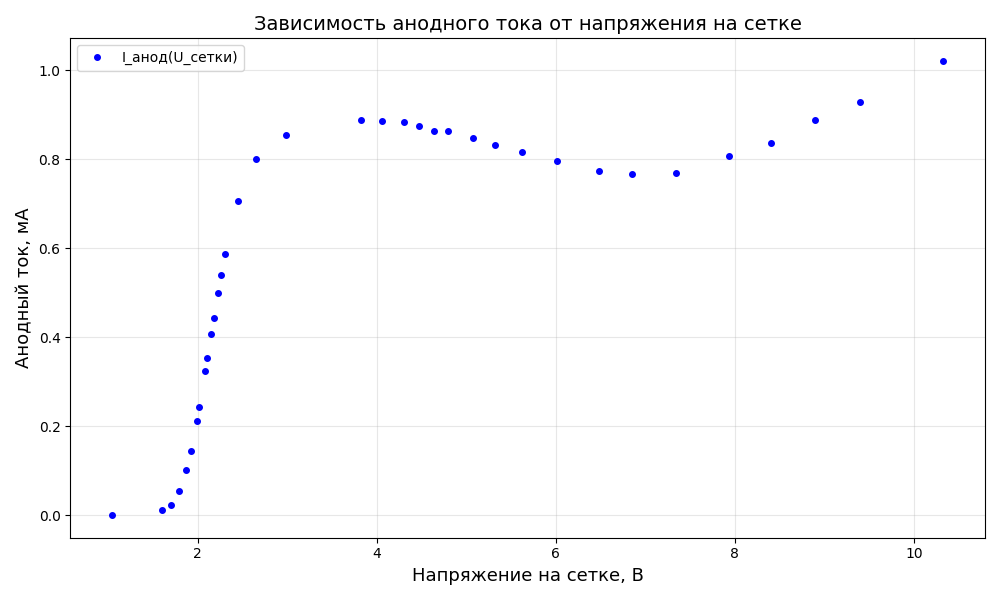
\includegraphics[width=0.6\textheight]{F2.png}
	\caption{Статический режим}
	\label{fig:screenshot3}
\end{figure}

\textbf{Вероятность рассеяния}

\[
w(V) = -\frac{1}{C} \ln \left( \frac{I_a(V)}{I_0} \right).
\]

Построим график зависимости $y = -ln(\frac{I_a}{I_0})$ от $V_c$:

\begin{figure}[tbh]
	\centering
	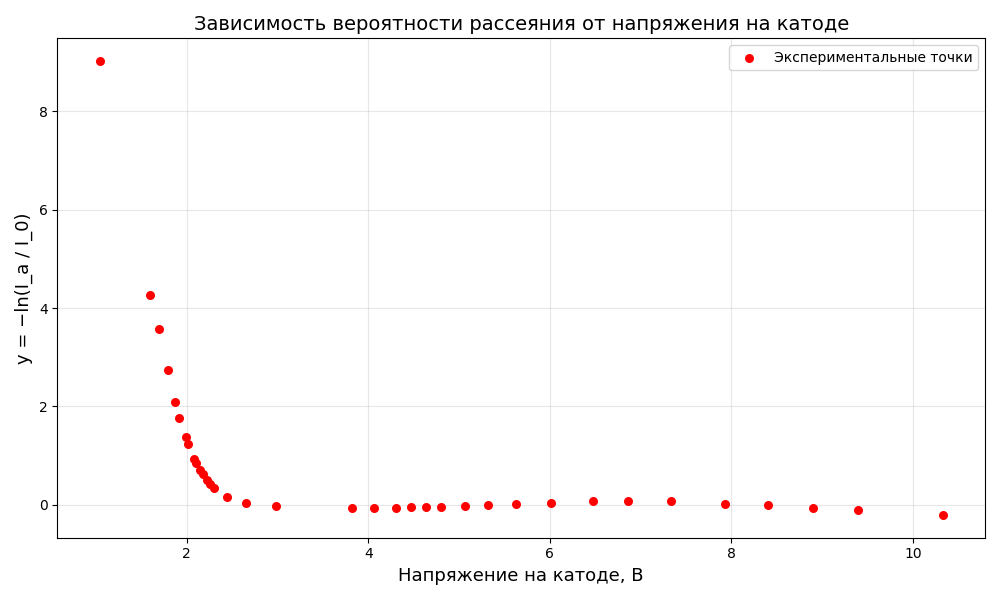
\includegraphics[width=0.5\textheight]{F3.png}
	\caption{Динамический режим}
	\label{fig:screenshot3}
\end{figure}

\textbf{Теоретический расчет для n=2,3}

Формула~(7): $k_2 l = n\pi$. Это условие резонанса (максимумов прохождения). Отсюда энергия:

\[
V_n = \frac{n^2 \pi^2 \hbar^2}{2 m_e e l^2} - U_0.
\]

$V_2$ = 18,1 \text{эВ}


$V_2$ = 43,9 \text{эВ}

\newpage

\section{Вывод}

В ходе данной работы был исследован эффект Рамзауэра, оценены параметры при разных режимах работы установки. Так, при помощи нескольких формул был оценён размер электронной оболочки атома, причём значения полученных оценок близки к табличному значению удвоенного ковалентного радиуса ($2{,}7$~\AA{}). Также было оценено значение потенциальной ямы, во всех опытах оно совпало по порядку, а в одном из даже оказалось достаточно близко к истинному. Также была получена зависимость вероятности рассеяния электронов от энергии, которая имеет поведения, похожее на график из методического материала.

\end{document}